\chapter{Case study}
\label{chap:case_study}

The goal of our case study introduced in this chapter is to show the application and an example of our hierarchical runtime verification framework. The motivation of this study was the related report from 2014 \citep{tdk2014}, where the goal was a distributed, model based security logic. The work of \citep{tdk2014} focused on the model driven development of a safety logic and its application in the Model Railway Project. Our work builds on the hardware and software presented in \citep{tdk2014} and extends it with the runtime verification of:
\begin{itemize}
	\item The safety logic in the embedded controllers.
	\item The correctness of the overall system.
\end{itemize}

\begin{figure}[h]
	\centering
	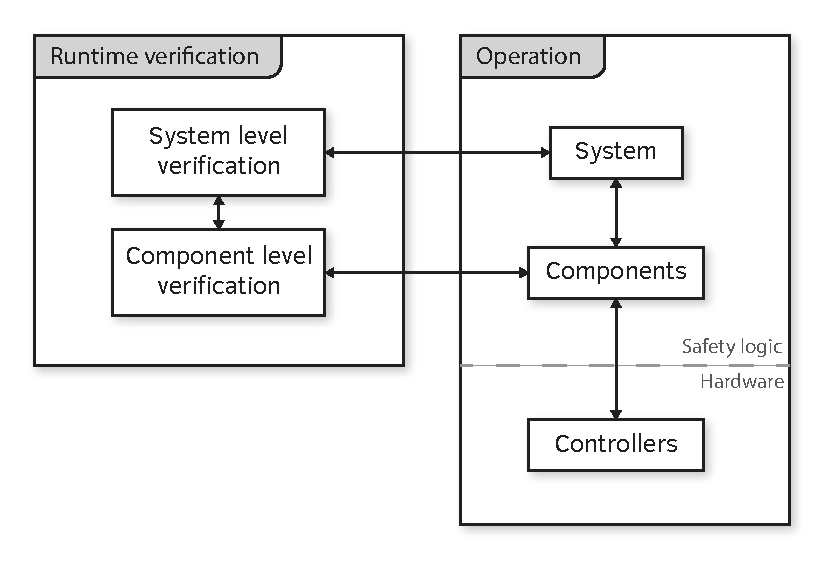
\includegraphics[width=0.65\linewidth]{include/figures/chapter_6/concept_1}
	\caption{The configuration of the case study}
	\label{fig:case_study:final_marker} 
\end{figure}

\section{System level observation with computer vision}

\subsection{Hardware}
\label{sec:case_study:hardware}

In case of a computer vision (\textls{CV}) based approach, it is critical to choose the appropriate hardware. We had two parameters in the selection of the camera: height above the board, and \textls{FOV}. The camera we used have these parameters:
\begin{itemize}
	\item Resolution: 1920x1080
	\item Horitontal FOV: \ang{120}
\end{itemize}

The camera have an installation height of $120$\si{\centi\meter}. This is a perfect value for using the case study in any room, and not suffer serious perspective distortions.

\subsection{OpenCV}

One key point of this study from the technological viewpoint is computer vision. It is a new extension of the hardware, which allows us to monitor the board with fairly big precision and reliability, if the correct techniques and materials are used.

We needed a fast, reliable, efficient library to use with the camera, and develop the detection algorithm. Our choice was the OpenCV\footnote{\url{http://opencv.org/}} library, which is an industry leading, open source computer vision library. It implements various algorithms with effective implementation e.g. using the latest streaming vector instruction sets. The main programming language -- and what we used -- is \textls{C++}, but it has many binding to other popular languages like Java, and Python.

\subsection{Marker design}

One of the steps of the \textls{CV} implementation was the design of the markers, which should provide an easy detection, and identification of the marked objects.

The first step was to consider the usage of an external library, named \textls{ArUco}\footnote{\url{http://www.uco.es/investiga/grupos/ava/node/26}}. This library provides the generation and detection library of markers. The problem with the library was the lack of tolerance in quality, and motion blur. Because these negative properties of the existing libraries, we implemented a marker detection algorithm for our needs.

After the implementation was in our hands, we could make markers which suits our needs. The chosen size of the markers was the size of the model railroad car's width as it provides the proper accuracy.

As explained in \cref{fig:case_study:opencv_math}, circular patterns are well suited for CV recognition applications. The final design consists of two detection circles, with a colored circle for the purpose of identification between them (\cref{fig:case_study:final_marker}).

\begin{figure}[h]
	\centering
	
\includegraphics[width=0.5\linewidth]{include/figures/chapter_6/opencv_finalmarker}
	\caption{The final marker design}
	\label{fig:case_study:final_marker} 
\end{figure}

\subsection{Mathematical solution for marker detection}
\label{fig:case_study:opencv_math}

%According to the various conditions, the marker detection has to be robust.

According to the various lighting conditions and used materials, the marker detection has to be robust. Also, the fact that these markers have perspective distortion when they are near the edges of the visible region of the camera, required the application of signal processing techniques.

This method is commonly used for transforming and processing a signal -- in our case a picture -- in the frequency domain.

\subsubsection{Convolution method}
\label{sec:case_study:convolution}

Our method is based on the convolution of two bitmap images, one from the camera, and one from the generated pattern.

According to the theorem, we can multiply two spectrums and apply an inverse Fourier transformation to get the convoluted image. If one image is the pattern, the other image is the raw\footnote{In our application raw (or raw image) means the unprocessed image from the camera}. Applying the convolution results in an image where every pixel represents the value how much the two spectrums match.

\subsubsection{Pattern bitmap properties}

The prerequisite for the pattern is that the size of the pattern and the size of the raw image must match, and the raw must be a grayscale image.

The pattern itself needs to be generated with values in accordance to the shape we would like to match (\cref{fig:case_study:convoluter_image}). The raw pixels are multiplied by this value. The meaning of the resulting values are the following: 
\begin{itemize}
	\item \bm{$value = 0$}: Doesn't affect the match.
	\item \bm{$value > 0$}: The multiplied raw pixel summed positively to the result of the convolution.
	\item \bm{$value < 0$}: The multiplied raw pixel summed negatively to the result of the convolution.
\end{itemize}

\begin{figure}[h]
	\centering
	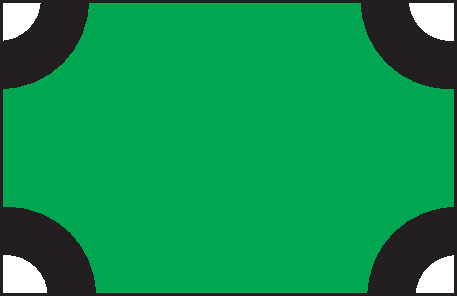
\includegraphics[valign=c,width=.5\linewidth]{include/figures/chapter_6/math_2}
	\rlap{\hspace{5pt}\begin{tabular}[c]{@{}cr@{}}
		\toprule
		\tikz \node [minimum width=1ex,minimum height=1ex,fill=black] {}; & $-1$ \\
		\tikz \node [minimum width=1ex,minimum height=1ex,fill=patternGreen] {}; & $0$ \\
		\tikz \node [minimum width=1ex,minimum height=1ex,fill=white,draw=black] {}; & $1$ \\
		\bottomrule
	\end{tabular}}
	\caption{Example for pattern bitmap placement and value}
	\label{fig:case_study:convoluter_image}
\end{figure}

\subsection{Software}

With the OpenCV library, we implemented a processing pipeline which can process the live video feed of the camera. The data is forwarded to the high level safety logic, which can decide what actions should be taken. The \cref{table:case_study:pipeline} shows all the essential steps in the processing pipeline of computer vision.

We used GPU acceleration through pipeline stage 1--4. The acceleration is implemented by OpenCV, and can be used with CUDA capable NVidia video accelerators.

\begin{table}[p]
	\caption{Computer vision processing pipeline}
	\label{table:case_study:pipeline}
	\centering
	\setlength{\fboxsep}{0pt}
	\setlength{\fboxrule}{1pt}
	\begin{tabularx}{\textwidth}{cm{5cm}X}
		\toprule
		Stage \# & Description & Example images  \\
		\midrule
		1 & Loading an image from the camera &\fbox{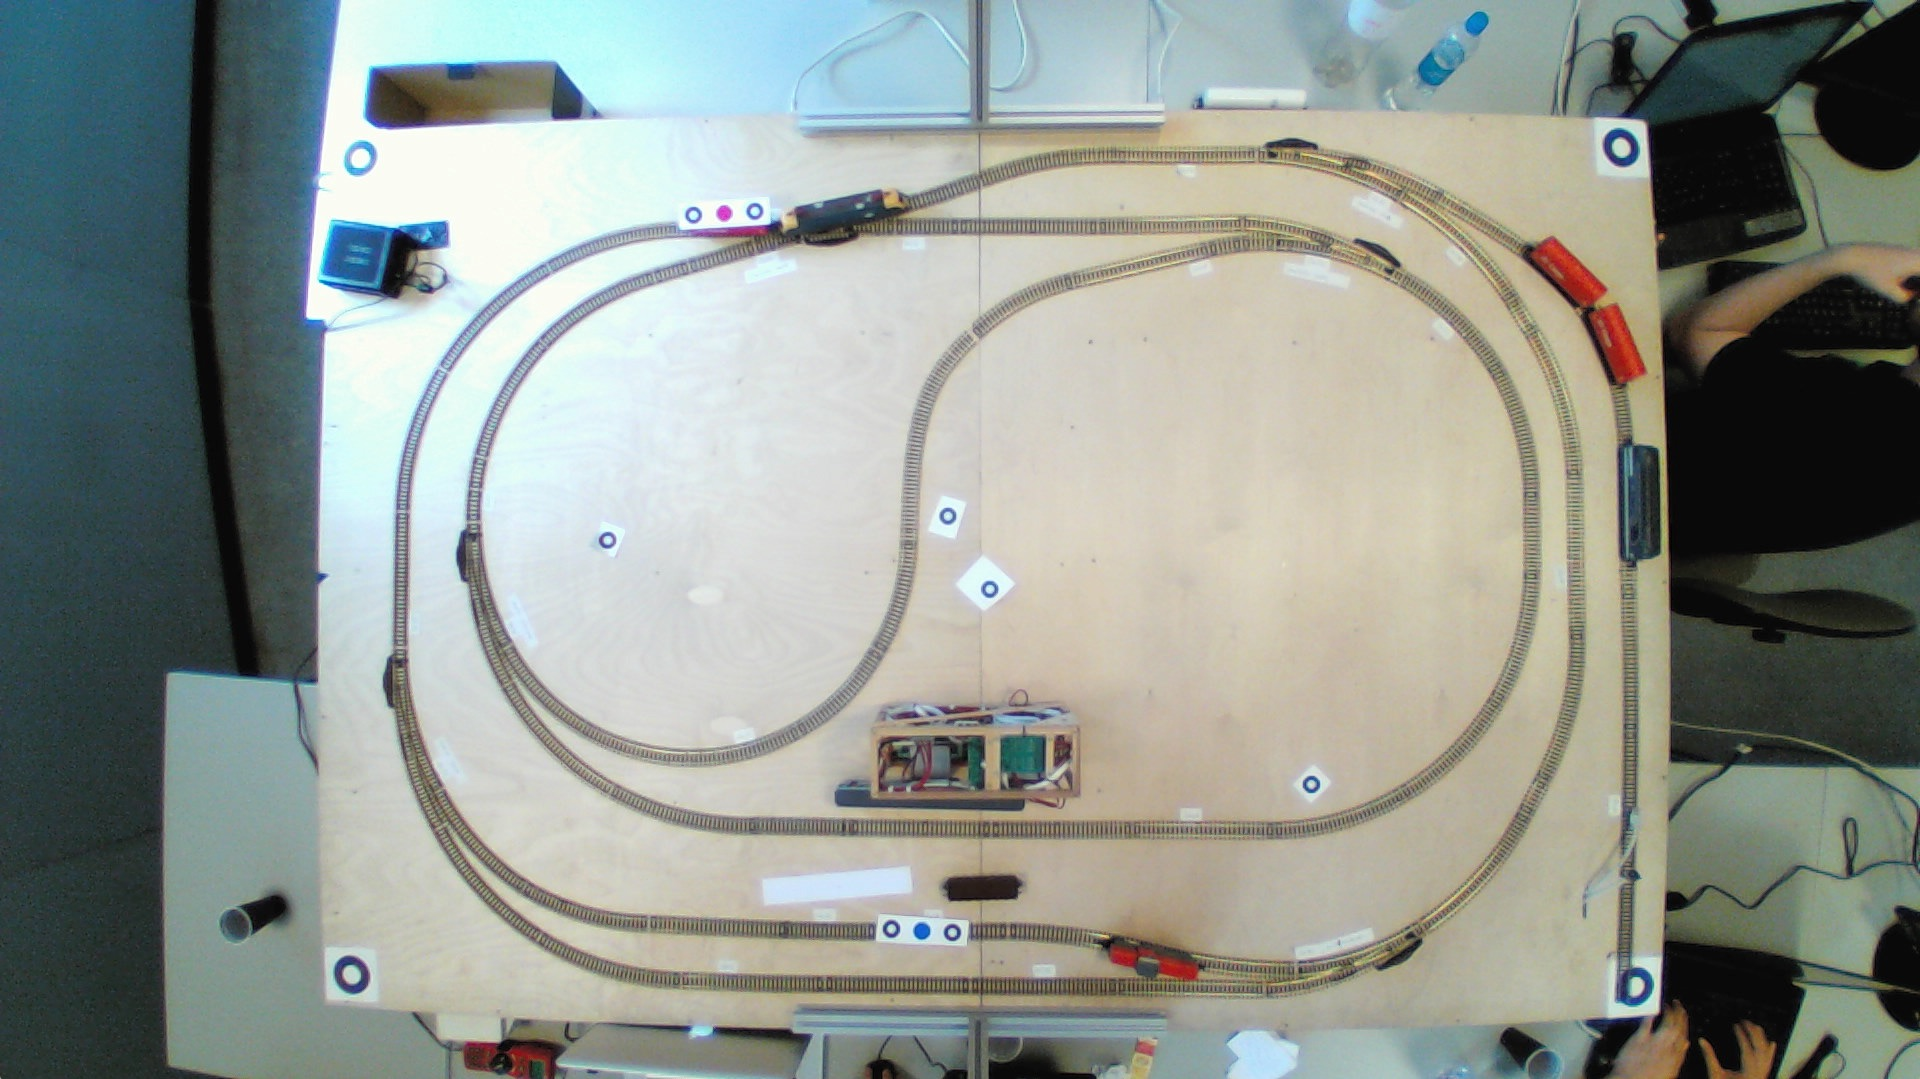
\includegraphics[valign=c,width=\linewidth]{include/figures/chapter_6/stages/s1}} \\[10.5ex]
		2 & Convert the image to grayscale & \fbox{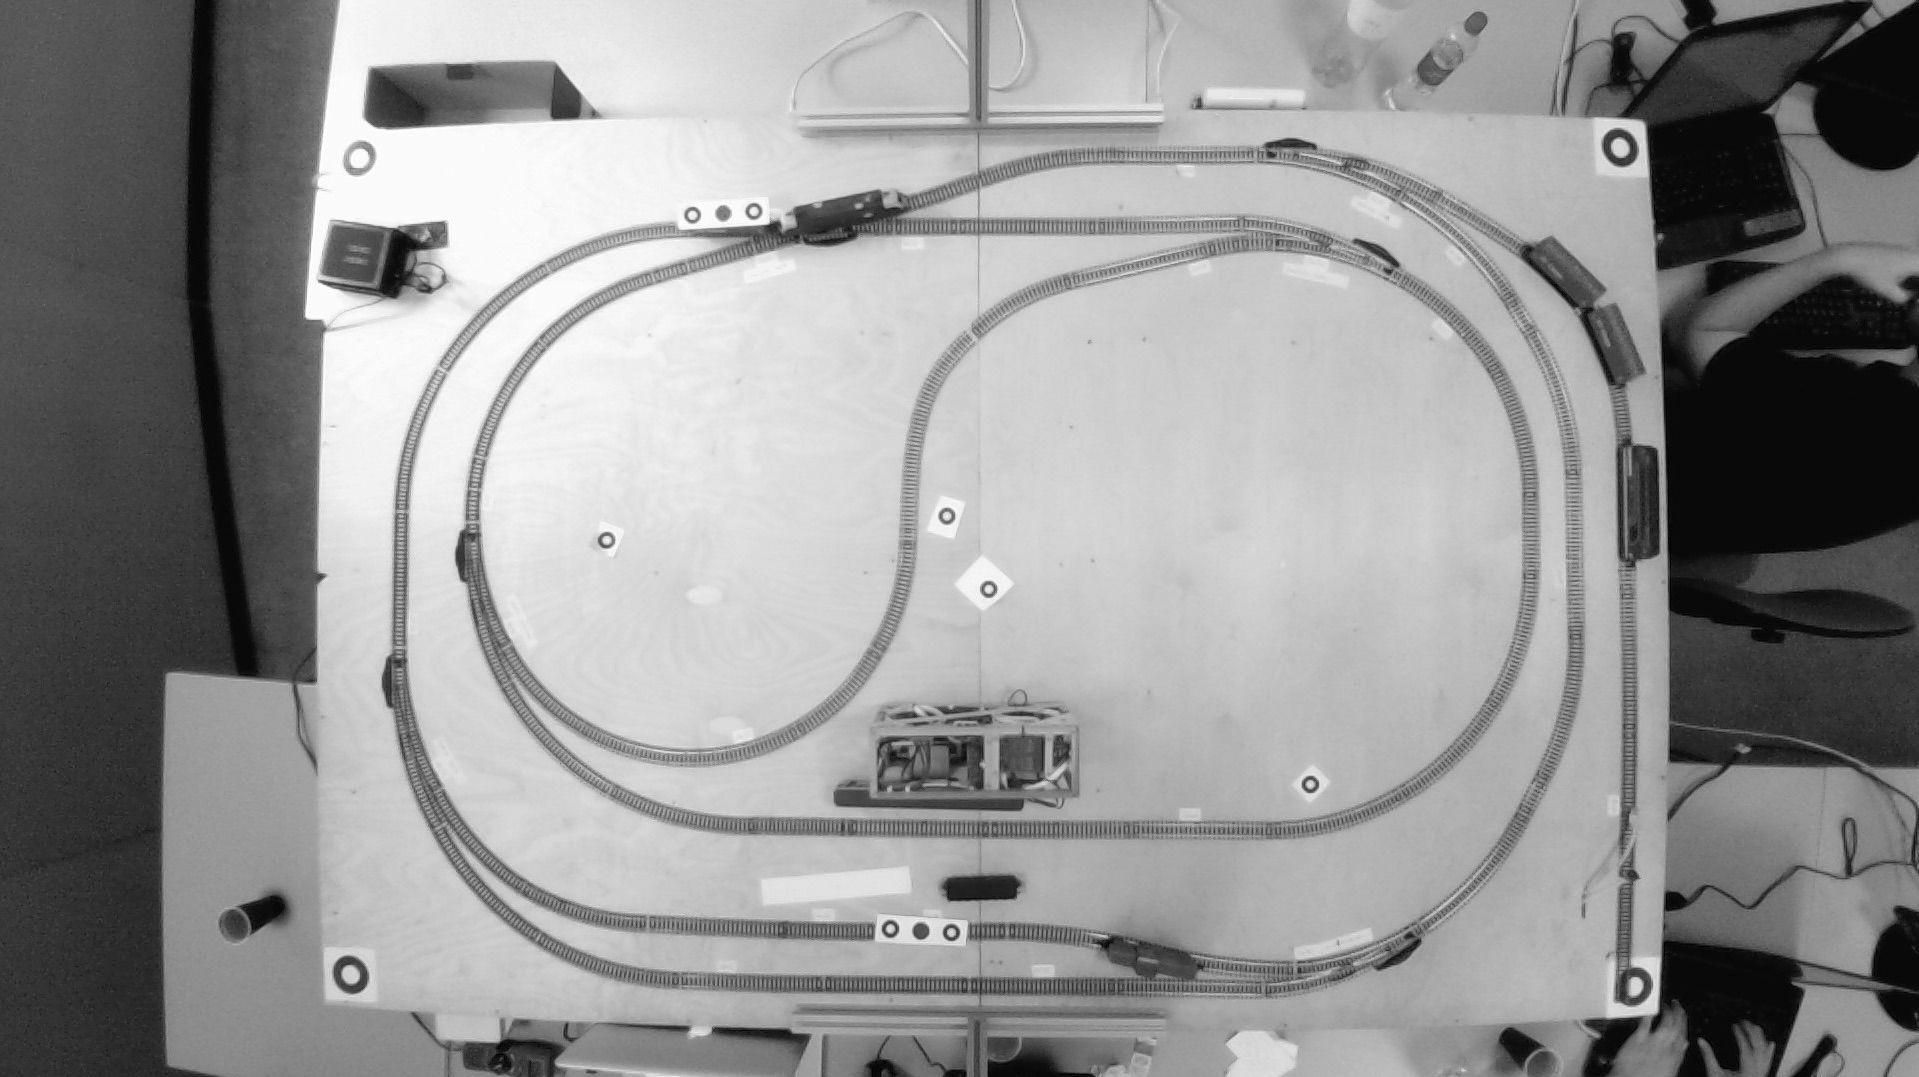
\includegraphics[valign=c,width=\linewidth]{include/figures/chapter_6/stages/s2}} \\[10.5ex]
		3 & Convolve the image with the pattern & \fbox{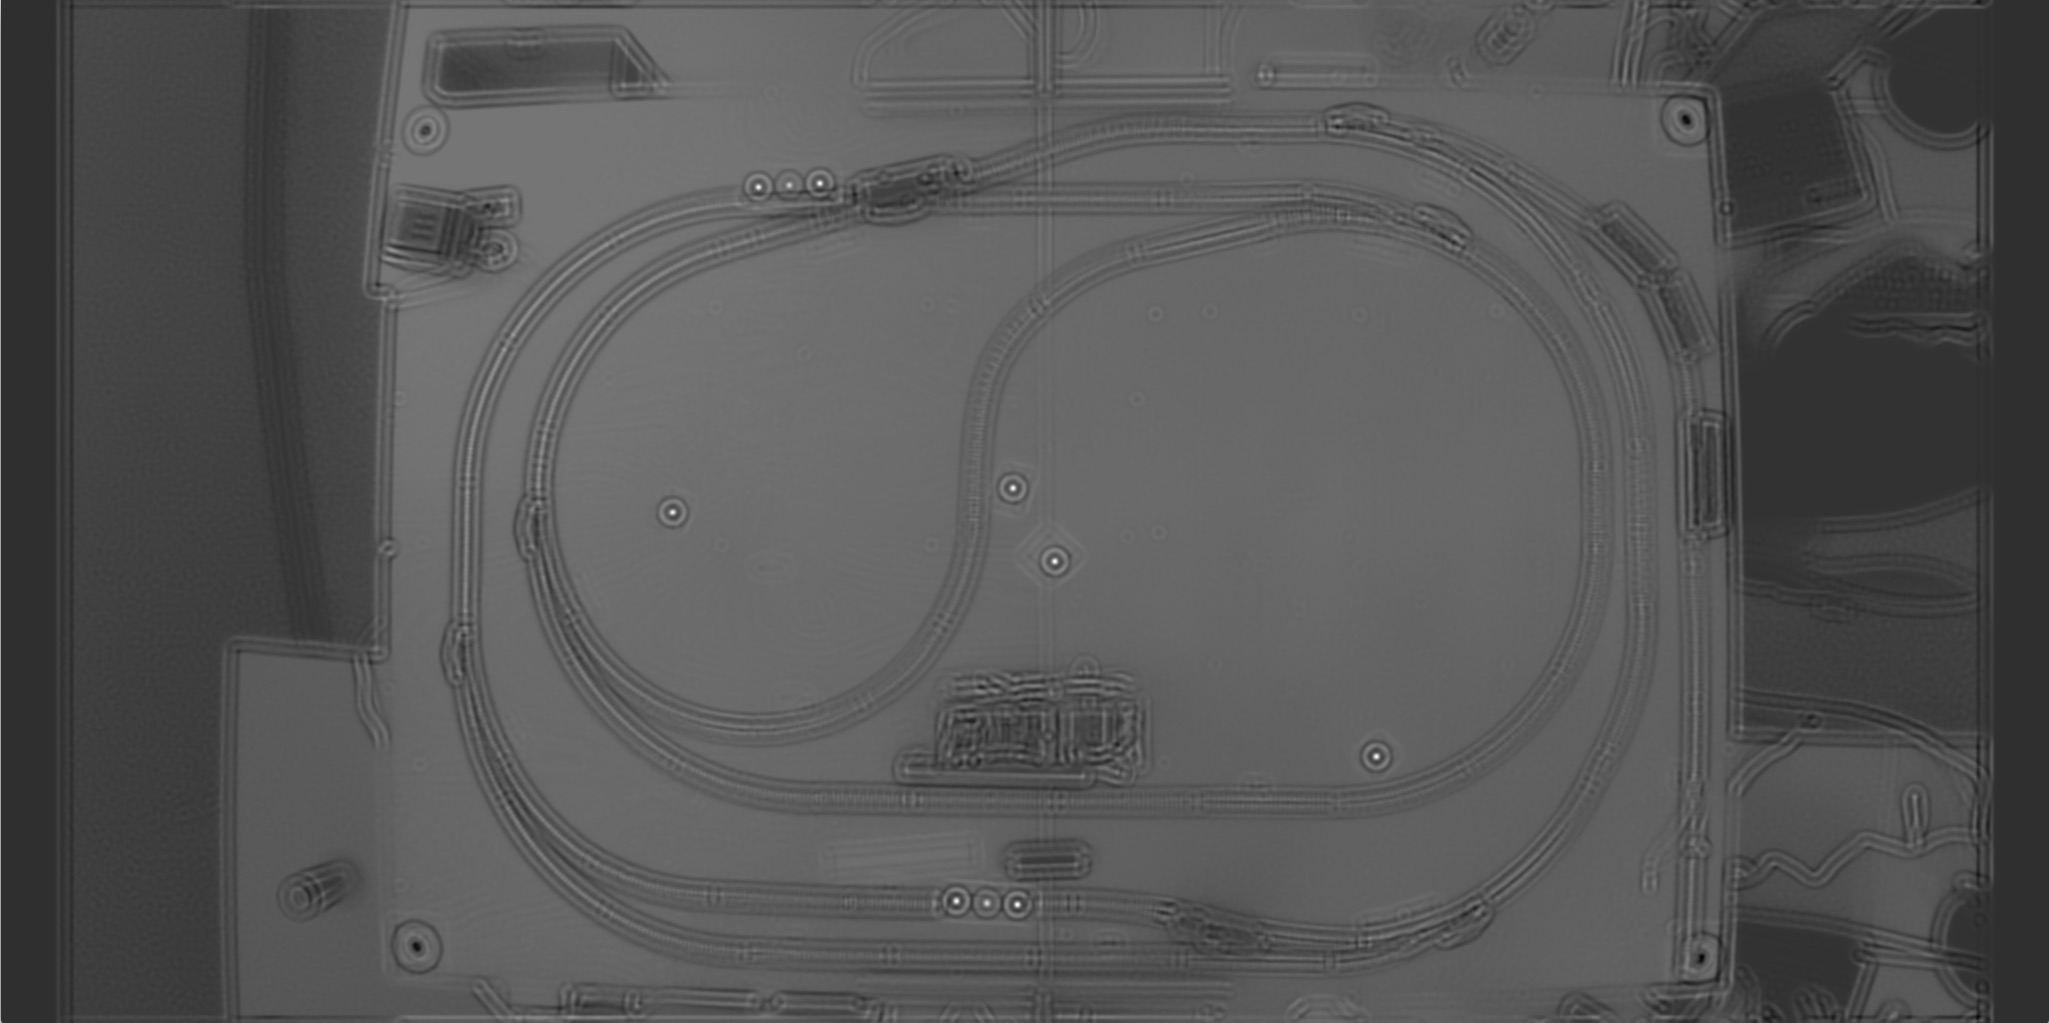
\includegraphics[valign=c,width=\linewidth]{include/figures/chapter_6/stages/s3}} \\[8.5ex]
	\end{tabularx}
	\begin{tabularx}{\textwidth}{cX}
		\toprule
		Stage \# & Description  \\
		\midrule
		4 & Applying a threshold to filter the brightest spots \\
		5 & Finding the contours of the enclosed shapes \\
		6 & Calculating the center point of the contours \\
		7 & Finding possible markers by distance \\
		8 & Identifying the marker by the center \\
		\bottomrule
	\end{tabularx}
\end{table}

\subsection{Summary}
With this implementation, we can follow the system in real-time, providing the high-level logic with an additional, independent source of information. This leads to a more robust system with added redundancy.

\newpage
\section{Model railroad}
In the following section, a briefly overview of the structure of the railroad and the controlling hardware is given.

\subsection{Overview}

\noindent The model railroad (\cref{fig:case_study:total_map}) contains the following hardware elements:
\begin{itemize}
	\item 15 powerable sections
	\item 6 railroad switchs
	\item 6 Arduino controllers for each switch
	\item 3 remotely controllable trains
\end{itemize}

\begin{figure}[h]
	\centering
	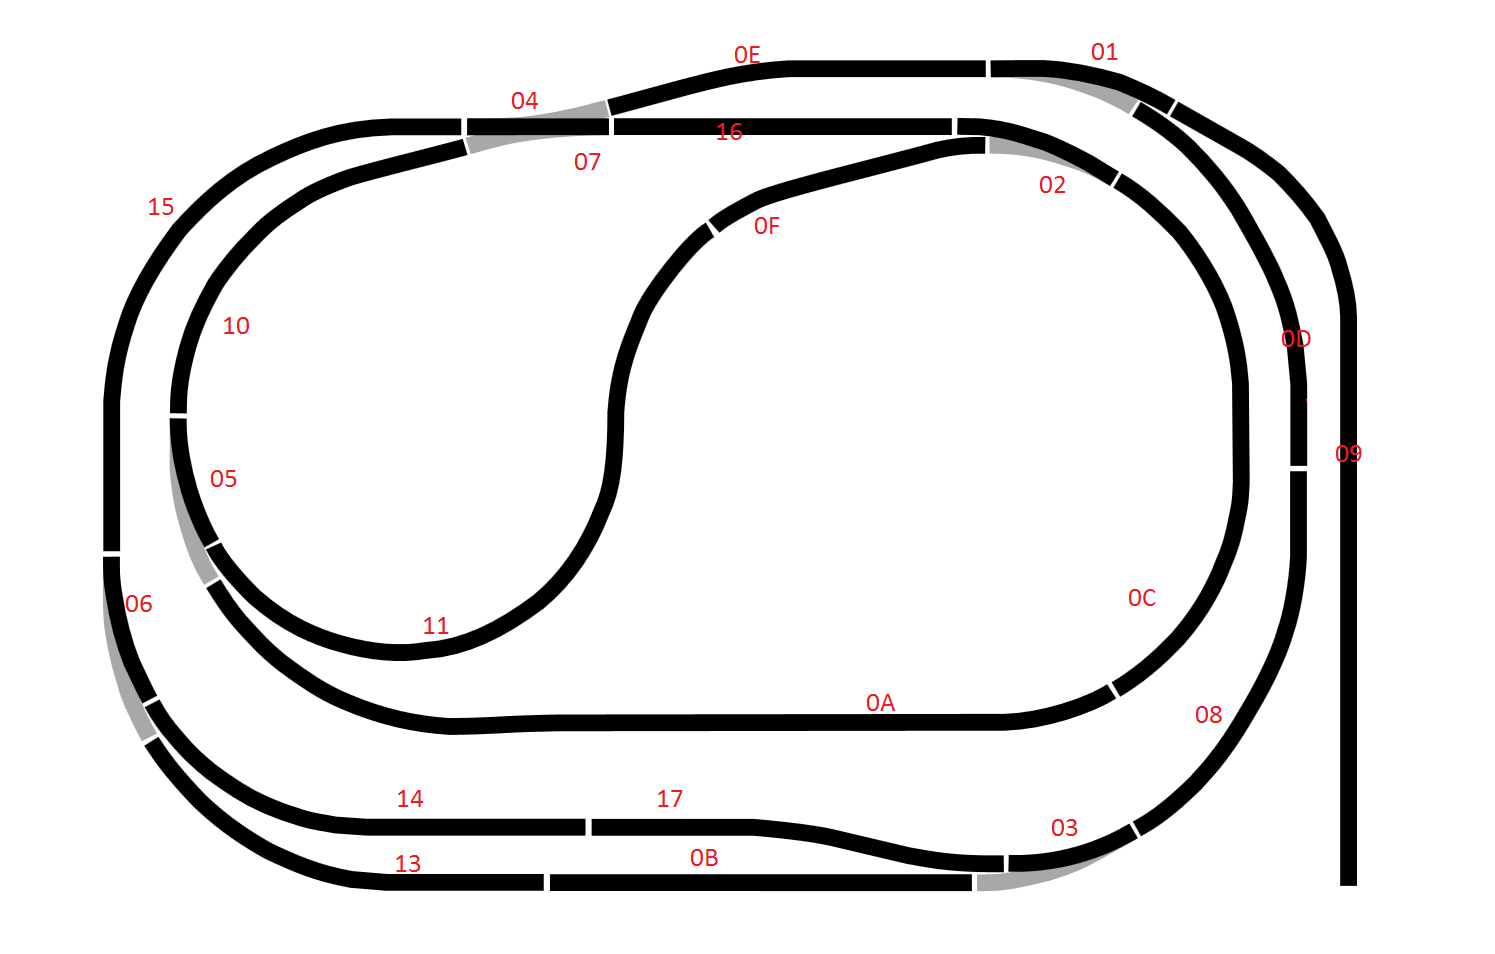
\includegraphics[width=\linewidth]{include/figures/chapter_6/total_view_1}
	\caption{The railroad network with section IDs}
	\label{fig:case_study:total_map}
\end{figure}

\subsection{Hardware}
The core of the hardware are the Arduino microcontrollers, which collect information and control the sections. For every railroad switch there is an associated controller which can control the power of the sections nearby, using the slave units connected to it (\cref{fig:case_study:master_slave}).

\begin{figure}[h]
	\centering
	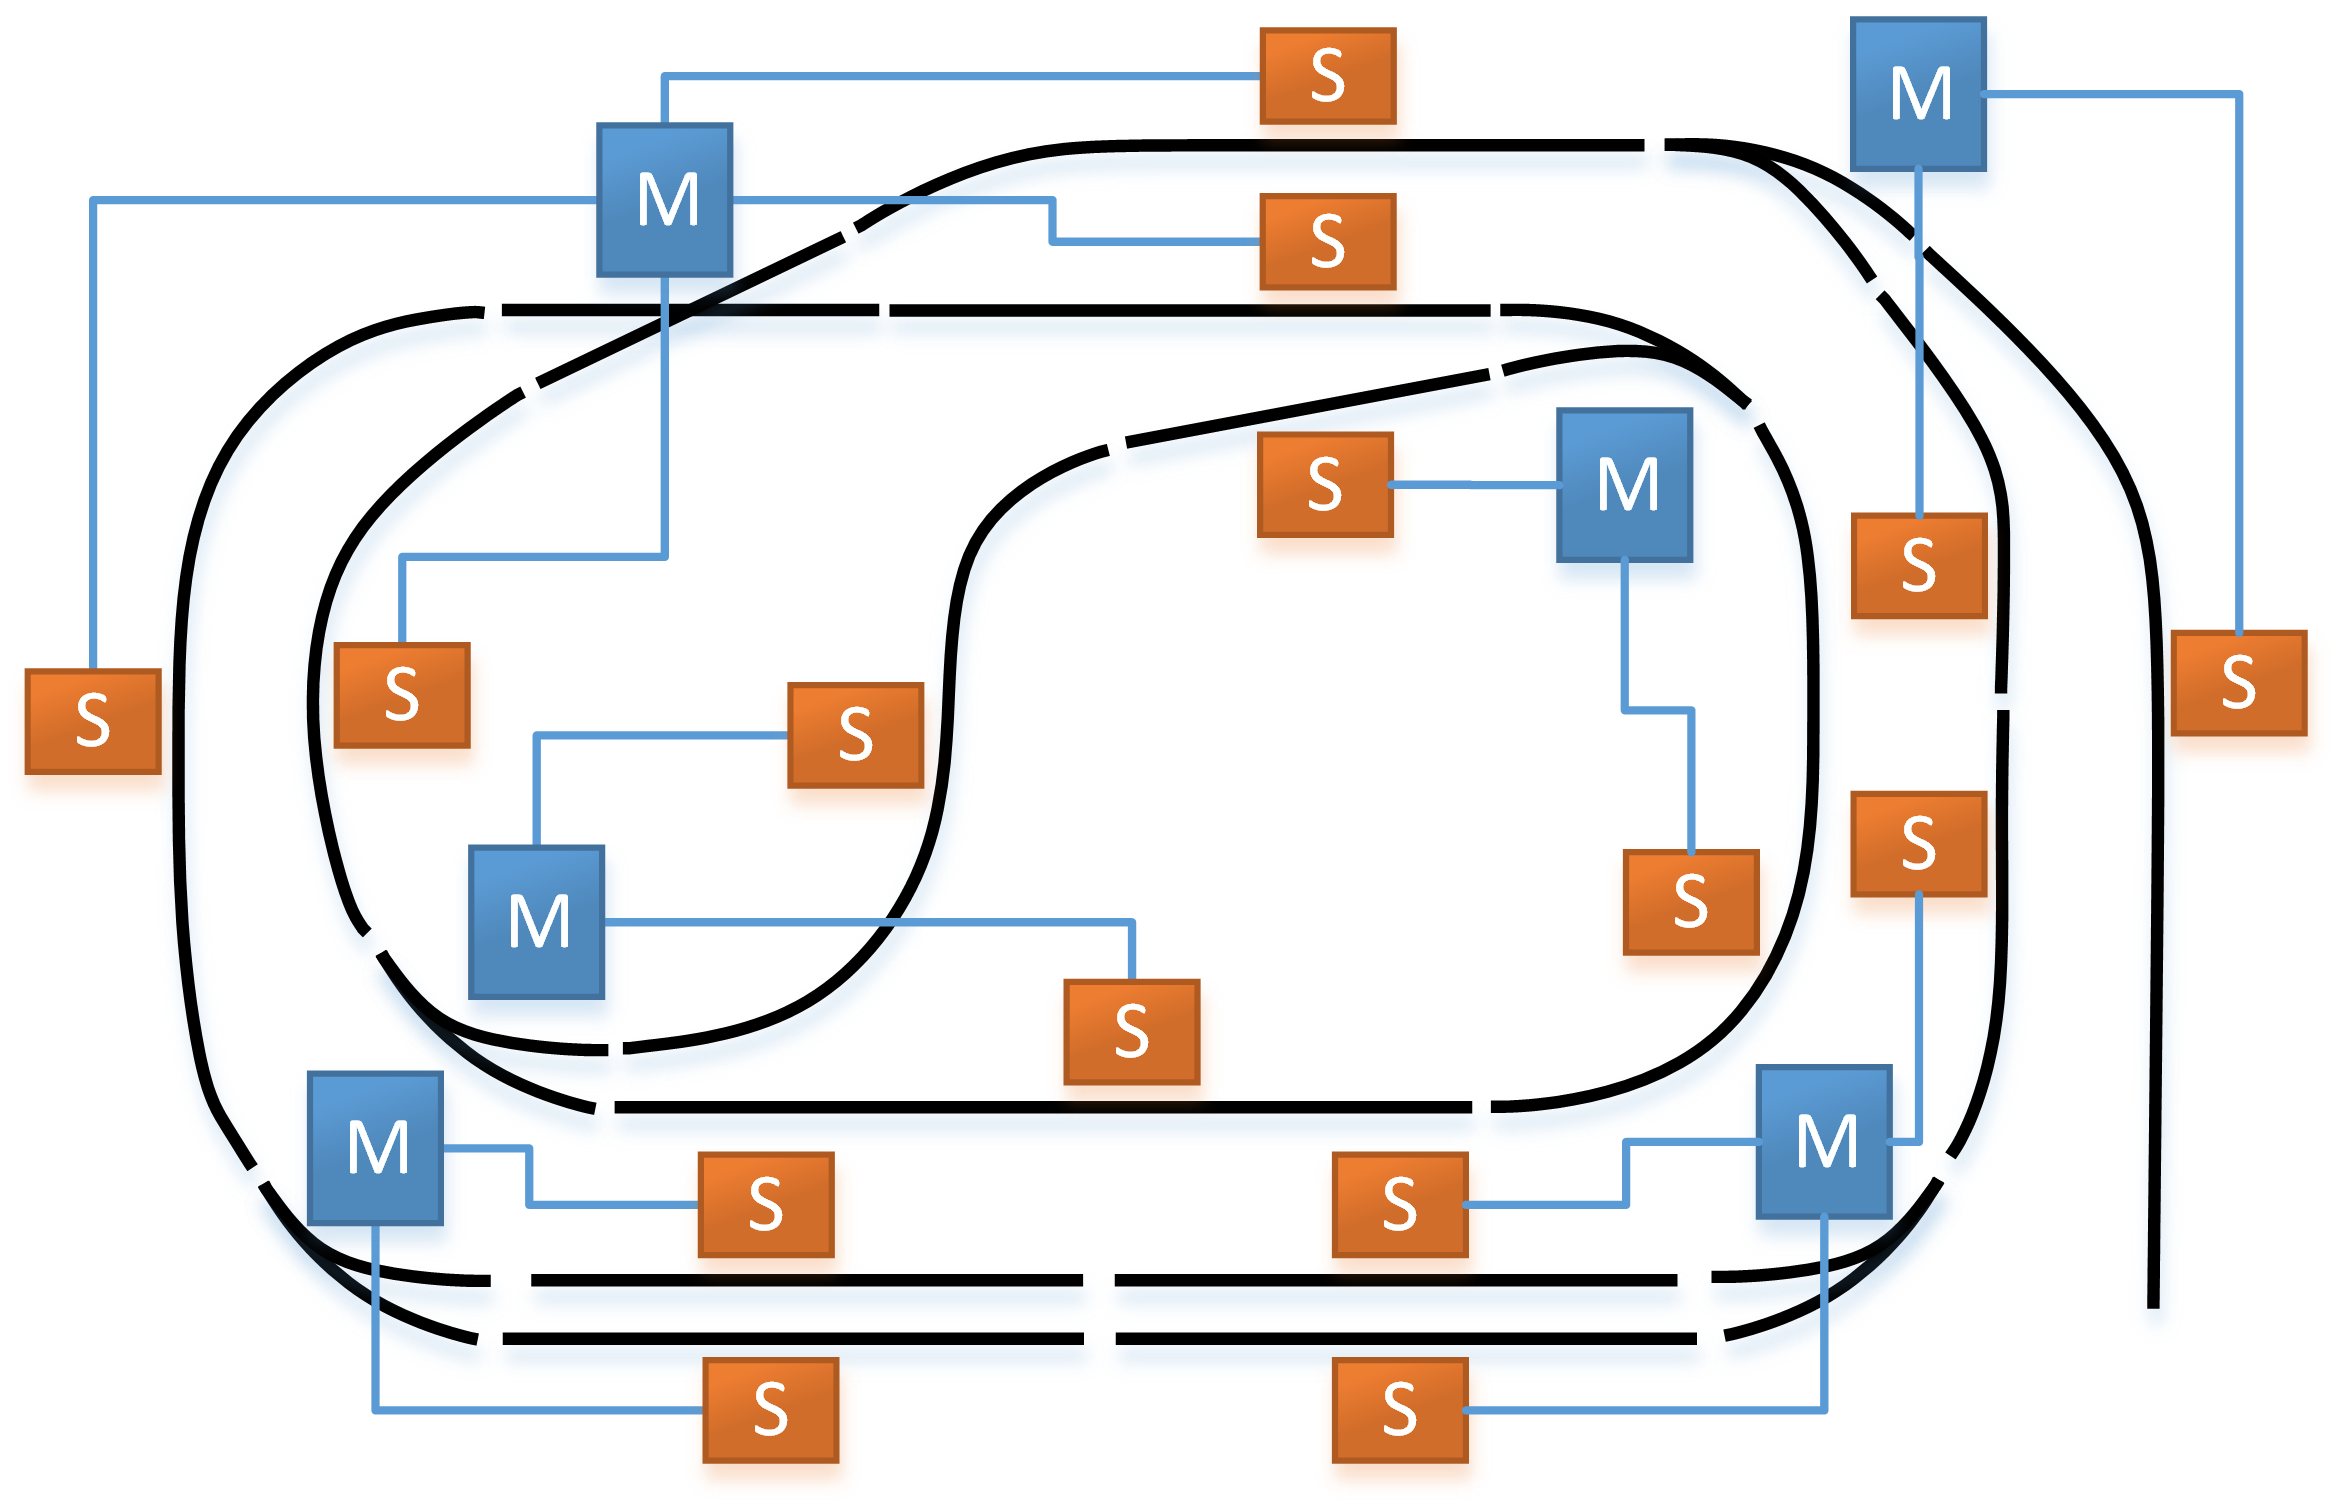
\includegraphics[width=\linewidth]{include/figures/chapter_6/railroad_ms}
	\caption{Master-slave associations}
	\label{fig:case_study:master_slave}
\end{figure}

\section{Metamodel design}
In this section we develop the metamodel of the system for the physical hardware. The safety logic is based on this logical model -- as a result, a model with many details of the physical world is needed.

\subsection{Physical elements}
The computer vision provides an external source of information for the system level logics. The CV forwards a train ID (determined by the marker color) and a position (x-y coordinates) to the model, and we must discretize this information in order to make it searchable by the safety logic for hazardous events.

The main components of the physical system are:
\begin{itemize}
	\item \textbf{Section}: Either a rail or a railroad switch. Every section has a distinctive identifier.
	\item \textbf{Rail}: A rail is a variable length curve. The main challenge is the determination of the next section. Only rails can be powered down, so the safety logic must act when the train is on a rail.
	\item \textbf{Railroad switch}: The switch is a region, where we know the entry and exit section by its setting. The switch is always powered, which means that the trains cannot be affected while on the switch. The basic concepts are:
	\begin{itemize}
		\item A switch consists of three rails: a central, a divergent and a straight rail.
		\item \textbf{Straight rail}: The straight rail follows the central rail without a curve.
		\item \textbf{Divergent rail}: The divergent rail moves away from the imaginary line of the central rail.
	\end{itemize}
\end{itemize}

\begin{figure}[h]
	\centering
	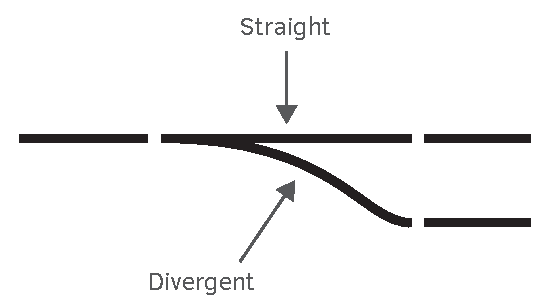
\includegraphics[width=0.5\linewidth]{include/figures/chapter_6/metamodel_switch_basics}
	\caption{The switch's straight, and divergent rails}
	\label{fig:case_study:metamodel_switch_basics}
\end{figure}

\begin{figure}[h]
	\centering
	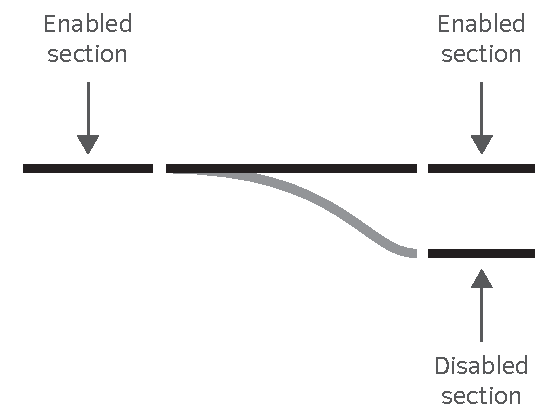
\includegraphics[width=0.5\linewidth]{include/figures/chapter_6/metamodel_switch_endi}
	\caption{Enabled-disabled section explanation}
	\label{fig:case_study:metamodel_switch_endi}
\end{figure}

\subsection{Metamodeling the physical elements}
\label{sec:case_study:logical_breakdown}
After specifying the physical elements and their properties, the logical concept of the model elements and their connections had to be uncovered.

A bottom-up structure was followed because it aids the graph search (\cref{sec:case_study:pattern_building}), and helps the review of the main components of the logical elements.

\begin{enumerate}
	\item \textbf{SectionModel}: The root of the board model. It is separated from trains as the root element is persisted, and loaded at every start of the application, while the \emph{TrainModel} is dynamic (\cref{fig:case_study:sectionmodel})(\cref{fig:case_study:trainmodel})(\cref{fig:case_study:groupmodel}).
	\begin{enumerate}
		\item \textbf{Configuration}: Contains the enabled \emph{groups} of the switch. The \emph{DivergentConfiguration} and \emph{StraightConfiguration} are exactly the same as the \emph{Configuration}. They are only presented in the metamodel because they allow the easier use of IncQuery patterns (\cref{sec:case_study:pattern_building}) (\cref{fig:case_study:settingmodel}).
		\item \textbf{SwitchSetting}: Contains a straight, and a divergent \emph{configuration} (\cref{fig:case_study:settingmodel}).
		\item \label{itm:case_study:region} \textbf{Region}: The atomic abstract element of the model. The \emph{region} is the smallest unit of measurement (\cref{fig:case_study:sectionmodel}).
		\item \textbf{SectionRegion}: Specialized region, which is a part of a \emph{powerable group}. Only powerable sections can stop a train (\cref{fig:case_study:sectionmodel}). 
		\item \textbf{RailRegion}: Specialized region. Because the exact position inside a switch is unessential, the entire area of the switch is declared as one region (\cref{fig:case_study:sectionmodel}).
		\item \label{itm:case_study:group} \textbf{Group}: A group is a collection of regions (\cref{fig:case_study:sectionmodel}).
		\item \textbf{PowerableGroup}: A collection of \emph{regions} which can be shut of. The equivalent to one rail in the modelled study (\cref{fig:case_study:sectionmodel}).
		\item \textbf{SwitchGroup}: A group of exactly one \emph{SwichRegion}. Has a reference to a \emph{Configuration}, describing the current switch settings (\cref{fig:case_study:sectionmodel}).
	\end{enumerate}
	\newpage
	\item \textbf{TrainModel}: The root of all train elements (\cref{fig:case_study:trainmodel}).
	\begin{enumerate}
		\item \textbf{Train}: The train representation with an unique ID, the current and previous region (\cref{itm:case_study:region}), and the next group (\cref{itm:case_study:group}) determined by the current, and previous region (\cref{fig:case_study:trainmodel}).
	\end{enumerate}
\end{enumerate}

\begin{figure}[H]
	\centering
	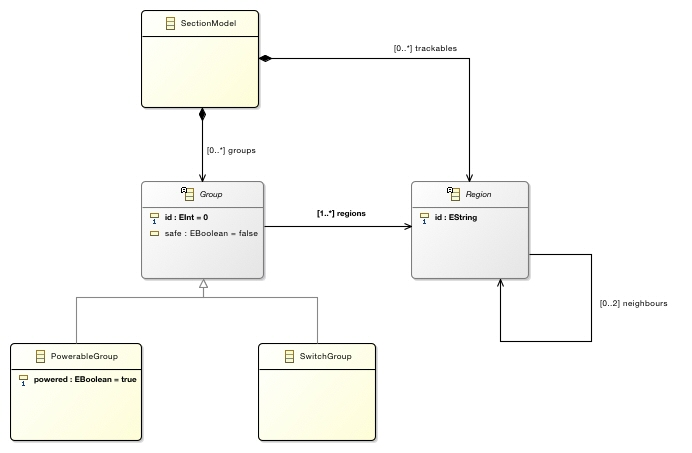
\includegraphics[width=1.2\linewidth]{include/figures/chapter_6/metamodels/groupmodel}
	\caption{The group view of the metamodel of the \emph{Model Railway Project} model} 
	\label{fig:case_study:groupmodel}
\end{figure}
\newpage
\begin{figure}[H]
	\centering
	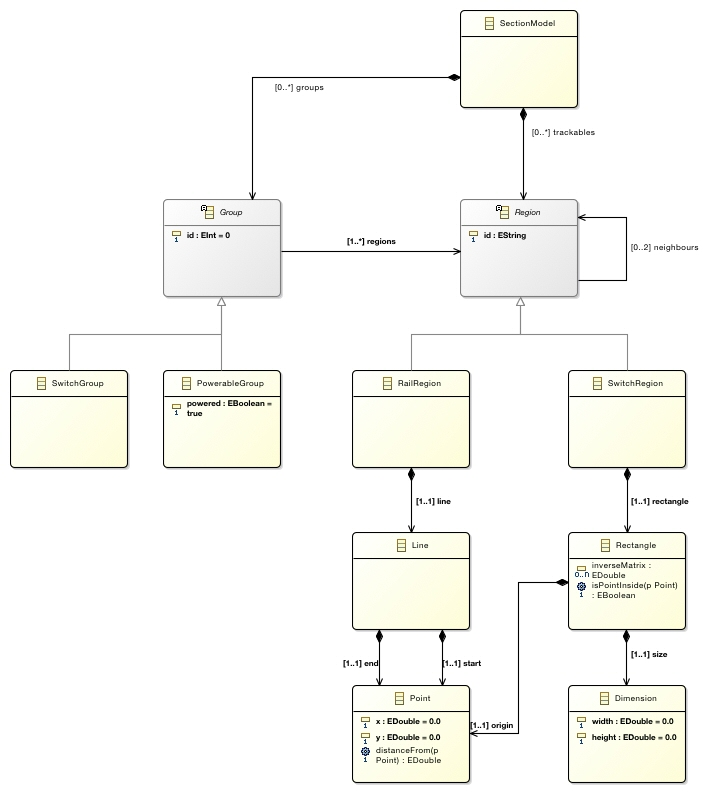
\includegraphics[width=1.2\linewidth]{include/figures/chapter_6/metamodels/sectionmodel}
	\caption{The section view of the metamodel of the \emph{Model Railway Project} model} 
	\label{fig:case_study:sectionmodel}
\end{figure}
\newpage
\begin{figure}[H]
	\centering
	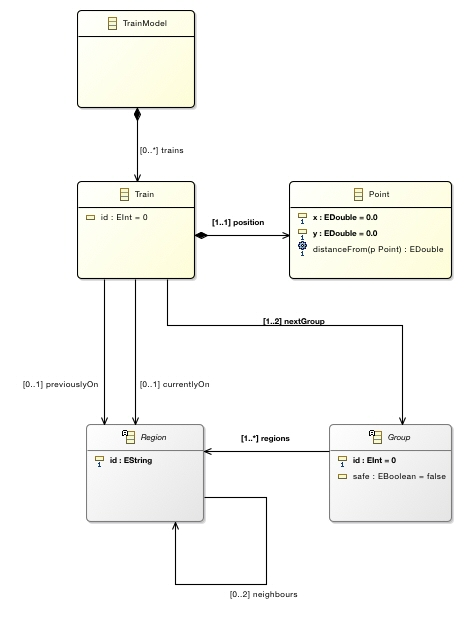
\includegraphics[width=1.0\linewidth]{include/figures/chapter_6/metamodels/trainmodel}
	\caption{The train view of the \emph{Model Railway Project} model} 
	\label{fig:case_study:trainmodel}
\end{figure}
\newpage
\begin{figure}[H]
	\centering
	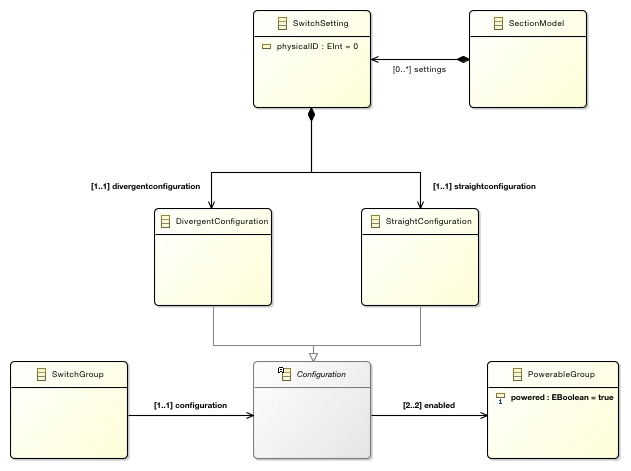
\includegraphics[width=1.2\linewidth]{include/figures/chapter_6/metamodels/settingmodel}
	\caption{The settings view of the \emph{Model Railway Project} model} 
	\label{fig:case_study:settingmodel}
\end{figure}

\newpage

\subsection{Using the Eclipse Modeling Framework}

We used EMF to develop the metamodel of the railway. The main reason for the usage of this modeling tool is that it allows the use of IncQuery. A few other reasons are:
\begin{itemize}
	\item Besides the POJO\footnote{Plain Old Java Object}, EMF can generate an Eclipse based editor for the model, where we can add/remove/edit all of the elements and their properties easily. The editor always checks the whether the model is well formed, and marks any problematic elements.
	\item The framework ensures that all of the used references are valid by updating them automatically.
	\item The declaration of opposing edges are also valid -- these are two-way references between objects. The framework will maintain these references e.g. if we assign object A to object B, if they have a bidirectional reference between them, the EMF will automatically update the other side of the reference, in our case the reference from A to B.
\end{itemize}

\subsection{Building the EMF model}

After the conceptual design of the model, the EMF model had to be designed.

When building EMF models, it is important that every element must be a part of exactly one containment tree. If an element is not in a tree or it is in multiple tree, the serialization process fails. In \cref{sec:case_study:logical_breakdown} the \emph{TrainModel} and \emph{SectionModel} represents the root of the model.

\subsection{Using EMF-IncQuery}

The motivation for the use of IncQuery is the graph based nature of the problem. The railway can be depicted as a graph, and hazardous patterns can be described e.g. a train's next section is the next section of an opposing train. These scenarios can be described declaratively by IncQuery patterns, reducing the possibility of a coding failure. 

The other advantage of using the IncQuery framework is it's scalability. The IncQuery framework -- as its name suggest: incremental query -- is a fast, caching query engine based on the RETE algorithm. The framework can effectively follow changes in huge environments. 

\subsection{Building the IncQuery patterns}
\label{sec:case_study:pattern_building}

Let us examine the patterns providing the essential filtering of hazardous patterns in the environment.
\\[1ex]

\begin{lstlisting}[caption={Collision detection},label=lst:case_study:train_will_collide]
pattern trainAtNextGroup(t1: Train) {
	Train.nextGroup(t1, ng);
	
	Train(t2);
	t1 != t2;
	
	Train.currentlyOn(t2, co);
	Group.regions(ng, co);
}
\end{lstlisting}

\cref{lst:case_study:train_will_collide} shows an IncQuery example. This pattern matches  the next group of \verb+t1+ -- if not null, e.g. the train is stationary -- which has a different train on it (\verb+t2+).

This example clearly represents the advantages of a declarative approach. With the right metamodel an incrementally executed scalable pattern can be designed with only 5 lines of code.
\\[1ex]

\begin{lstlisting}[caption={Collision detection},label=lst:case_study:train_at_next_powerable]
pattern trainAtNextPowerable(t1: Train) {
	Train.nextGroup(t1, ng);
	Train.currentlyOn(t1, t1co);
	
	SwitchGroup(ng);
	SwitchGroup.configuration.enabled(ng, enabled);
	enabled != t1co;
	
	Train(t2);
	t1 != t2;
	Train.currentlyOn(t2, t2co);
	Group.regions(t2g, t2co);
	
	enabled == t2g;
}
\end{lstlisting}

\newpage
\cref{lst:case_study:train_at_next_powerable} is a pattern for finding the next powerable group in the direction of travel. This is a necessity as trains cannot stop on switch groups. With \cref{lst:case_study:train_will_collide} hazardous situations in the next group can be filtered, but if the train is on a switch, it might crash. This pattern is specialized in the case of a train going towards a switch. The other side of the switch is examined. If any train is present, the pattern will match, switching the power off the section.
\\[1ex]

\begin{lstlisting}[caption={Collision detection},label=lst:case_study:train_at_next_powerable]
pattern trainFromDisabled(t: Train) {
	SwitchGroup(sg);
	SwitchGroup.regions(sg, region);
	SwitchGroup.configuration.enabled(sg, enabled);
	region != enabled;
	
	Train.currentlyOn(t, region);
	Train.nextGroup(t, sg);
}
\end{lstlisting}

\section{Component-monitor integration}

The related study \citep{tdk2014} implemented a model based security logic. With the use of the statechart language presented in \vref{chap:runtime_verification}, we can monitor the state and execution of the model, and verify it on a higher level. In this example, we break the execution of the safety logic into two parts:
\begin{itemize}
	\item \textbf{Monitoring the execution engine}: Execution errors (entry to error states) are detected by the monitors. The resolution of the monitoring is set to 1 second.
	\item \textbf{Monitoring the transitions of the model}: If the safety logic cannot access it's sensors, or communicate, the model execution will stop because of the lack of input. This behavior can be detected.
\end{itemize}

\begin{figure}[h]
	\centering
	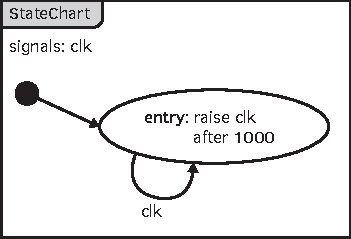
\includegraphics[width=0.3\linewidth]{include/figures/chapter_6/statecharts/clock}
	\caption{Clock generation state chart}
	\label{fig:case_study:clockgen}
\end{figure}

\subsection{Monitor statecharts}
\label{sec:case_study:mon_sc}

\begin{figure}[h]
	\centering
	\begin{minipage}{0.49\linewidth}
		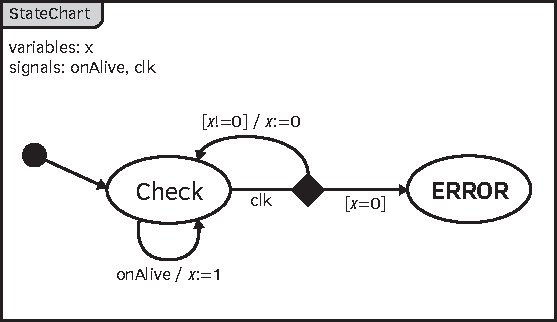
\includegraphics[width=0.9\linewidth]{include/figures/chapter_6/statecharts/onalive}
	\end{minipage}
	\begin{minipage}{0.49\linewidth}
		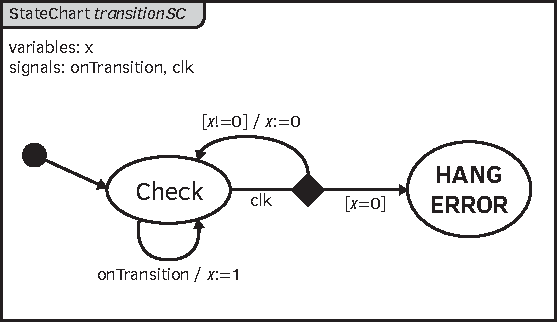
\includegraphics[width=0.9\linewidth]{include/figures/chapter_6/statecharts/ontransition}
	\end{minipage}
	\caption{Error detection state machines}
	\label{fig:case_study:errors}
\end{figure}

\cref{fig:case_study:clockgen}, and \cref{fig:case_study:errors} show the concept of our monitor statechart. The statechart \emph{clockGen} generates a periodic clock sign of 1\si{\second}. In the statecharts \emph{aliveSC} and \emph{transitionSC} we use this clock signal as a timing event. If the expected signals are not triggered between two clock cycles, the statechart steps into an error state.

\begin{lstlisting}[caption={Statechart representation of clock generation},label=lst:case_study:clk_gen]
specification transitionSpec {
    signal clk
    statechart clockSC {
        region clockSC {
            initial state i
            state clock {
                entry: raise clk after 1000
            }
            transition from clock to clock on clk
        }
    }
}
\end{lstlisting}

\newpage
\begin{lstlisting}[caption={Statechart representation of hang error detection},label=lst:case_study:hang_error]
specification transitionSpec {
    signal clk
    signal onTransition
    statechart transitionSC {
        local x : integer
        region transitionSC {
            initial state i
            state Check
            state HangError
            choice errorDetection
            transition from i to Check
            transition from Check to errorDetection on clk
            transition from errorDetection to HangError [x=0]
            transition from errorDetection to Check [x/=0] / assign x:=0
            transition from Check to Check on onTransition / assign x:=1
        }
    }
}
\end{lstlisting}

\begin{lstlisting}[caption={Statechart representation of hang error detection},label=lst:case_study:hang_error]
specification aliveSpec {
    signal clk
    signal onAlive
    statechart aliveSC {
        local x : integer
        region aliveSC {
            initial state i
            state Check
            state ExecError
            choice errorDetection
            transition from i to Check
            transition from Check to errorDetection on clk
            transition from errorDetection to ExecError [x=0]
            transition from errorDetection to Check [x/=0] / assign x:=0
            transition from Check to Check on onAlive / assign x:=1
        }
    }
}
\end{lstlisting}

\newpage
\subsection{Generated VEPL}

The statecharts' definitions from \cref{sec:case_study:mon_sc} generates a VEPL pattern for the system monitor component, therefore we can write patterns, and define actions for pattern matches.

\begin{lstlisting}[caption={Generated VEPL definition},label=lst:case_study:gen_vepl]
package hu.bme.mit.tdk2015.critcyber.vepl

AtomicEvent ExecError(id: String)
AtomicEvent HangError(id: String)
\end{lstlisting}

\nohyphenation The generated stub (\cref{lst:case_study:gen_vepl}) contains the error states of the statechart as AtomicEvents. With these events, a complex event processing pattern can be built.
\\[1ex]

\begin{lstlisting}[caption={Extended VEPL definition},label=lst:case_study:ext_gen_vepl]
package hu.bme.mit.tdk2015.critcyber.vepl

AtomicEvent ExecError(id: String)
AtomicEvent HangError(id: String)

rule ExecErrorRule on ExecError {
	System.out.println("Error source id: " + ruleInstance.atom.parameterTable.parameterBindings.head.value);
	ErrorHandler::handleExecError(ruleInstance.atom.parameterTable.parameterBindings.head.value)
}

rule HangErrorRule on HangError {
	System.out.println("Error source id: " + ruleInstance.atom.parameterTable.parameterBindings.head.value);
	ErrorHandler::handleHangError(ruleInstance.atom.parameterTable.parameterBindings.head.value)
}
\end{lstlisting}

With \cref{lst:case_study:ext_gen_vepl}, a very simple pattern is used to match the generated events, and handle them by defining rules without any conditions. Events can be parametrized, so an event itself can mark the source of the validation error. The \verb+ErrorHandler+ class is needed because the model cannot be accessed from the rule, therefore a static class is needed which can modify the state of the model. For example, if the static method \verb+handleHangError+ sets the \verb+safe+ attribute of the \verb+Group+ with the id we can fetch from the event representing the error state, the \cref{lst:case_study:trainReachUnsafe} pattern can match.

\newpage
\begin{lstlisting}[caption={Collision detection},label=lst:case_study:trainReachUnsafe]
pattern trainReachUnsafe(t: Train) {
	Train.nextGroup(t, ng);
	Group.safe(ng, safe);
	check(safe == false);
} or {
	Train.currentlyOn(t, co);
	Group.regions(g, co);
	
	Train.nextGroup(t, ng);
	PowerableGroup(ng);
	find regionNeighbour(ng, nng);
	nng != g;
	
	Group.safe(nng, nng_safe);
	nng_safe == true;
} or {
	Train.currentlyOn(t, co);
	Group.regions(g, co);
	
	Train.nextGroup(t, ng);
	SwitchGroup(ng);
	SwitchGroup.configuration.enabled(ng, enabled);
	enabled != g;
	
	Group.safe(enabled, nng_safe);
	nng_safe == true;
}
\end{lstlisting}

This pattern filters those trains whose second next track is unsafe. The middle rail is needed for buffering because we cannot be sure about the unsafe track state (\cref{fig:case_study:unsafe}), and if another train is coming in the opposing direction, there is a chance that it cannot be stopped. As a result, the insertion of the middle track is a necessity to prevent collisions (\cref{fig:case_study:safe}). This is an example of runtime verification: we get notified about the component failures, and the higher level logic can act before the catastrophe.

\newpage
\begin{figure}[H]
	\centering
	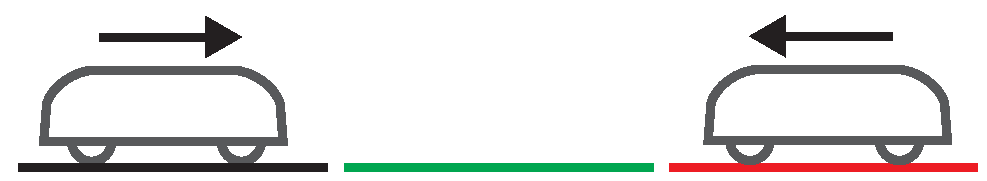
\includegraphics[width=0.7\linewidth]{include/figures/chapter_6/failsafe/safe}
	\caption{Safe configuration. The train from the failed group can be stopped on the buffer rail.}
	\label{fig:case_study:safe}
\end{figure}

\begin{figure}[H]
	\centering
	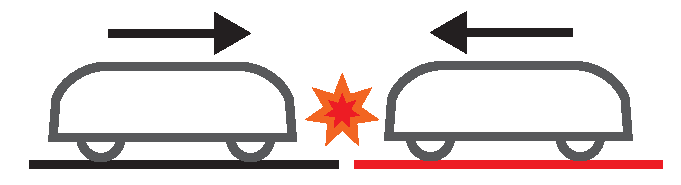
\includegraphics[width=0.5\linewidth]{include/figures/chapter_6/failsafe/unsafe}
	\caption{Unsafe configuration. If a train comes in the opposing direction, they will crash.}
	\label{fig:case_study:unsafe}
\end{figure}

\section{Summary}

The Train Benchmark\cite{TrainBenchmark} shows a similar railroad application with IncQuery based pattern matching. Their benchmark showed IncQuery can match patterns on a similar railroad model with element sizes over 80 million under 100 milliseconds after the initial caching.
